\Annex{Entrelacement d'insertions concurrentes dans Treedoc}

\label{app:treedoc-interleaving}

\begin{figure}[!ht]

  \centering
  \resizebox{\columnwidth}{!}{
    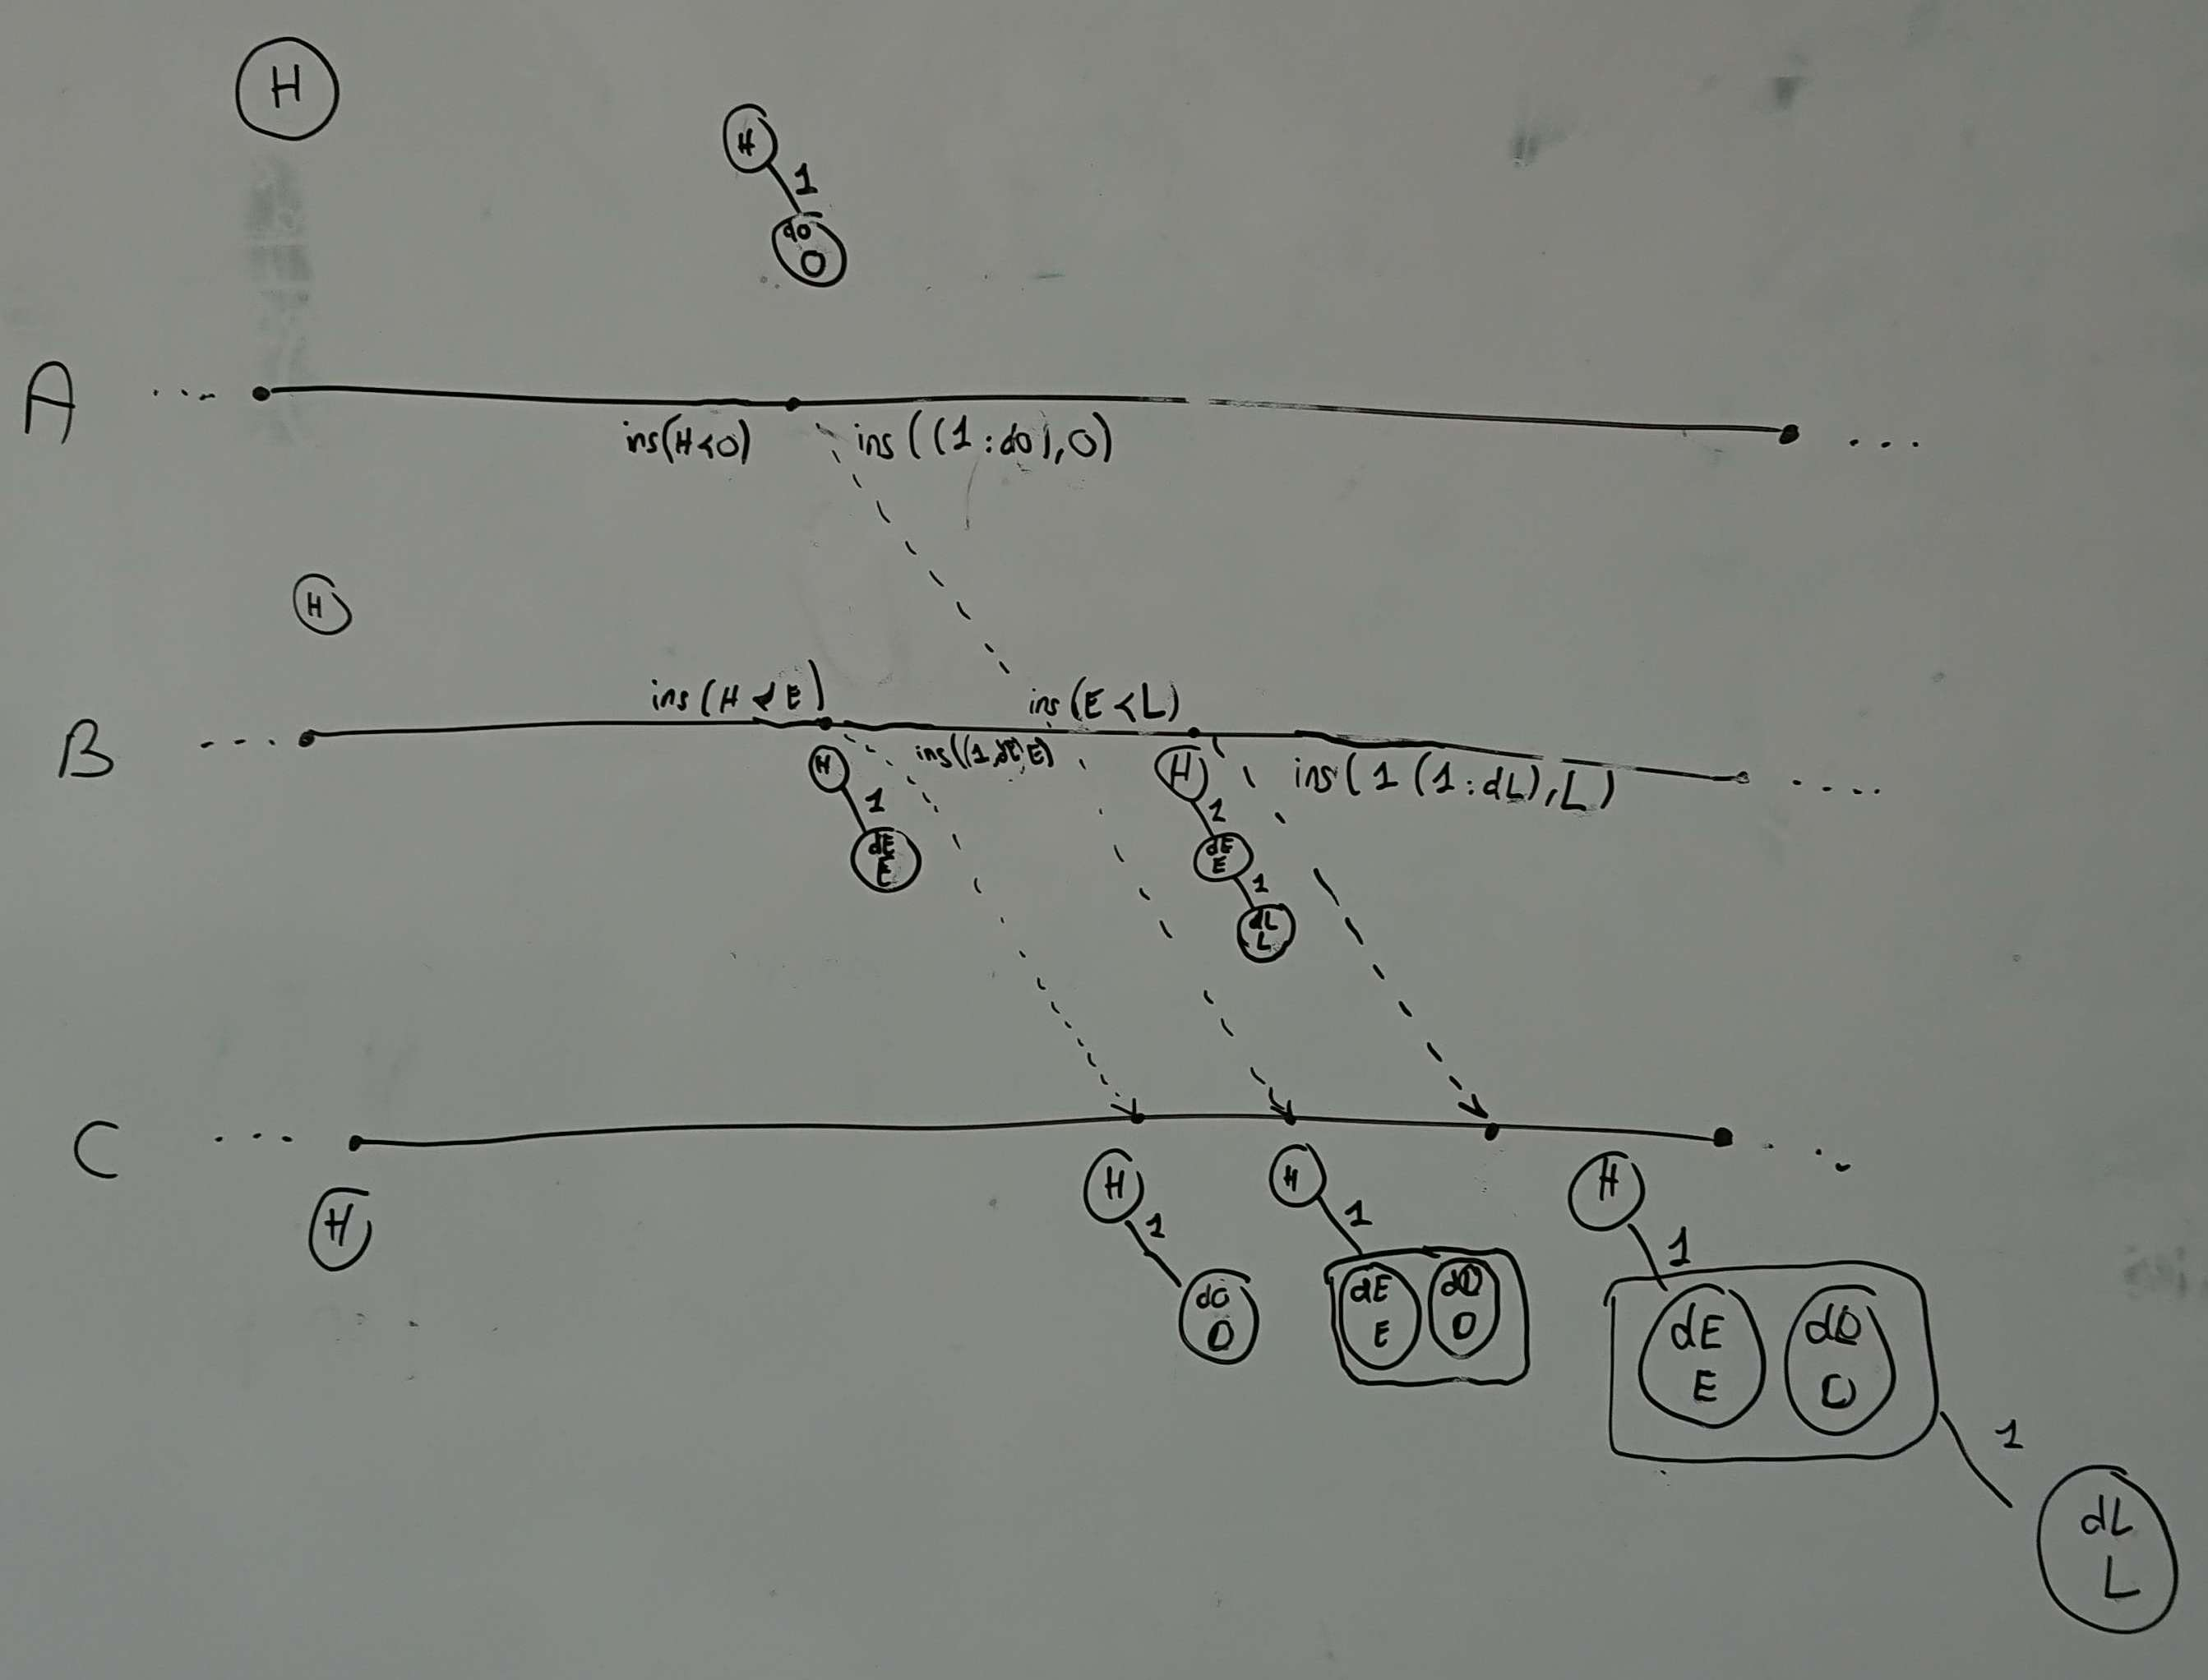
\includegraphics{img/contre-exemple-treedoc}
  }
  \caption{Modifications concurrentes d'une séquence Treedoc résultant en un entrelacement}
\end{figure}

\mnnote{
  TODO: Réaliser au propre contre-exemple.
  Nécessite que $d_E < d_O$, inverser A et B histoire d'éviter toute confusion.
  En soi, C pas nécessaire, à voir si le conserve.
}
